\documentclass[a4paper,10pt]{article}
\usepackage[utf8]{inputenc}
\usepackage[T1]{fontenc}
\usepackage[english,italian]{babel}
\usepackage[hmargin=2cm,vmargin=2cm, bottom=2cm]{geometry}
\usepackage{fancyhdr}%
\usepackage{amsfonts}
\usepackage{graphicx}
\usepackage[ruled]{algorithm2e}
\usepackage{titling}
\usepackage[normalem]{ulem}

\setlength{\droptitle}{-5em}   % This is your set screw
\pagestyle{fancy}% Change page style to fancy
\fancyhf{}% Clear header/footer
\fancyhead[C]{Michele Lazzeri | 822879}
\fancyfoot[C]{\thepage}% \fancyfoot[R]{\thepage}
\renewcommand{\headrulewidth}{0.4pt}% Default \headrulewidth is 0.4pt
\renewcommand{\footrulewidth}{0.4pt}% Default \footrulewidth is 0pt
\setlength{\parindent}{0pt}

%inizio custom commands
\newcommand{\entita}[1]{\textsc{\textbf{#1}}}
\newcommand{\assoc}[1]{\textit{#1}}
\newcommand{\relaz}[1]{\textsc{\textbf{#1}}}
\newcommand{\attr}[1]{\textsf{#1}}
\newcommand{\key}[1]{\uline{#1}}
\newcommand{\fkey}[1]{\textit{#1}}
%fine custom commands

\title{Progetto di Basi di Dati - Documentazione Tecnica}
\author{Michele Lazzeri | 822879}
\date{}

\begin{document}
\maketitle
\section{Progettazione Er}
Da una prima analisi del testo lo schema er iniziale risulta essere:

\centerline{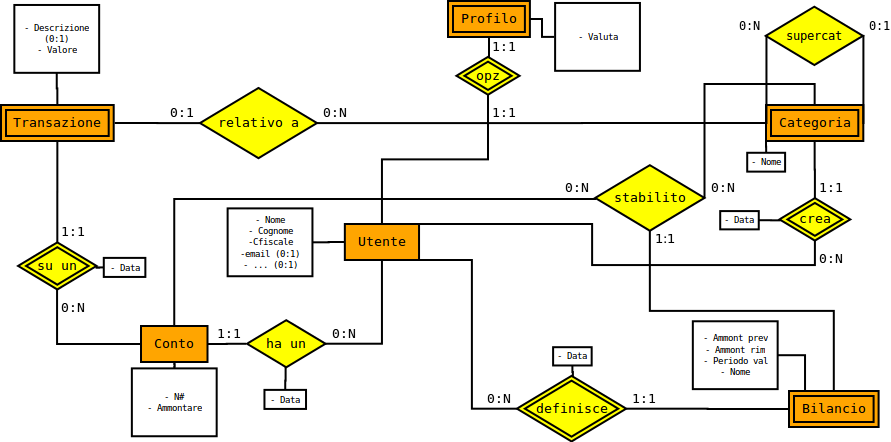
\includegraphics[scale=0.65]{ER.png}}




Di queste sono considerate tipi di entità deboli (entità in cui la chiave è definita da un associazione con un altra entità):
\begin{itemize}
\item \entita{Transazioni} la cui chiave è formata da un ID e dal numero del conto relativo, quest'ultimo derivante dall'associazione \assoc{Su\_{}un}
\item \entita{Categoria} la cui chiave è formata dal nome della categoria e dall'identificatore dell'utente che l'ha creata, quest'ultimo derivante dall'associazione \assoc{crea}
\item \entita{Bilancio} la cui chiave è formata dal nome del bilancio e dall'identificatore dell'utente che l'ha definito, quest'ultimo derivante dall'associazione \assoc{definisce}
\item \entita{Profilo} la cui chiave è formata dall'identificatore dell'utente che l'ha definito, derivante dall'associazione \assoc{opz}
\end{itemize}

Per quanto riguarda le gerarchie abbiamo le seguenti suddivisioni:
\begin{itemize}
\item \entita{Conto} viene suddivisa tramite gerarchia Totale Esclusiva in: \begin{itemize}\item\entita{Deposito} \item\entita{Credito}: \attr{Tetto\_{}Massimo\_{}Credito, Periodo Rinnovo, Data Iniziale}
\end{itemize}
\item \entita{Transazioni} viene suddivisa tramite gerarchia Totale Esclusiva in: \begin{itemize}\item\entita{Spesa}\item\entita{Entrata}\end{itemize}
\item \entita{Categoria} viene suddivisa tramite gerarchia Totale Esclusiva in : \begin{itemize}\item\entita{Categoria di spesa}\item\entita{Categoria di Entrata}\end{itemize}
\end{itemize}

\section{Ristrutturazione}
Nella prima fase della ristrutturazione vengono analizzati i dati derivati: in questo caso:
\begin{itemize}
\item \attr{Ammontare} di Conto e Bilancio vengono mantenuti anche se calcolabili a partire dalle spese: essendo la query 'Dammi il saldo del conto x' molto comune risulta molto più veloce l'accesso a tale informazione se contenuta direttamente in un'entità rispetto al calcolo di tale valore tramite somma di tutte le spese/entrate associate a tale entità.
\end{itemize}

Quindi vengono eliminate le gerarchie:
\begin{itemize}
\item \entita{Conto}: viene riunita in una sola entita \entita{Conto} in quanto spese, entrate e bilanci possono essere associate indistintamente a Conti di Credito o Conti di Debito. Viene quindi aggiunto l'attributo \attr{Tipo} all'entità
\item \entita{Transazioni}: vengono mantenute solo le sottoclassi, in quanto  i bilanci sono definiti solo per le spese
\item \entita{Categoria}: vengono mantenute le sottoclassi, in quanto non avrebbe senso suddividere le spese e le entrate e mantenere unite le relative categorie
\end{itemize}


Quindi vengono definiti gli identificatori primari:
\begin{itemize}
\item \entita{Conto}: Numero (creato perchè non esiste un insieme di attributi abbastanza ridotto da poter essere utilizzato in modo efficace)
\item \entita{Spesa}: Id\_{}operazione e Conto.Numero
\item \entita{Entrata}: Id\_{}operazione e Conto.Numero
\item \entita{Categoria}: Nome e Utente.ID
\item \entita{Bilancio}: Nome e Utente.ID
\item \entita{Utente}: Userid (creato perchè non esiste un insieme di attributi abbastanza ridotto da poter essere utilizzato in modo efficace)
\item \entita{Conto}: Utente.Userid
\end{itemize}
Note:
\begin{itemize}
\item l'idea di tenere suddivisi Profilo e Utente nonostante abbiano la stessa chiave è quella di suddividere le informazioni relative all'utente come Persona Fisica (dati ''reali'') e le informazioni utilizzate dall'applicazione

\end{itemize}

Quindi vengono eliminati gli attributi multivalore o composti:
in questo schema non ne sono presenti

Alla fine della ristrutturazione lo schema ER si presenta come segue:

\centerline{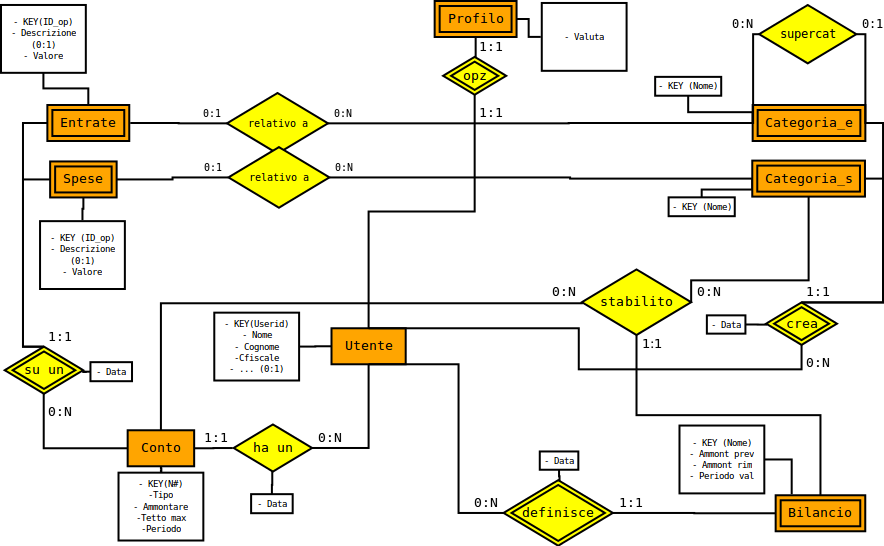
\includegraphics[scale=0.65]{ERpost.png}}

\section{Traduzione}
La traduzione da ER a Modello Relaziona porta al seguente schema relazionale:
\begin{itemize}
\item[]\entita{conto} (\attr{\key{Numero}}, \attr{amm\_{}disp}, \attr{tipo}, \attr{tettomax}, \attr{scadenza\_{}giorni}, \attr{\fkey{utente}}, \attr{datacreazione}, \attr{\fkey{conto\_{}di\_{}rif}})

\item[]\entita{spesa} (\attr{\key{\fkey{conto}, id\_{}op}},  \attr{data, \fkey{cat\_{}s\_{}nome, cat\_{}s\_{}user}, descrizione, valore})

\item[]\entita{entrata} (\attr{\key{\fkey{conto}, id\_{}op}},  \attr{data, \fkey{cat\_{}e\_{}nome, cat\_{}e\_{}user}, descrizione, valore})

\item[]\entita{categoria\_{}spesa} (\attr{\key{\fkey{utente}, nome}, supercat\_{}nome})
\item[]\entita{categoria\_{}entrata} (\attr{\key{\fkey{utente}, nome}, supercat\_{}nome})

\item[]\entita{bilancio} (\attr{\key{\fkey{utente}, nome}, ammontareprev, ammontarerest , periodovalidita, datapartenza})

\item[]\entita{utente} (\attr{\key{userID}, nome, cognome, email, indirizzo, cfiscale, citta, datadinascita, comunedinascita, nazioneresidenza, telefono})

\item[]\entita{profilo} (\attr{\key{\fkey{utente}}, valuta})

\item[]\entita{bilancio\_{}conto} (\attr{\key{\fkey{bilancio.utente, bilancio.nome, conto}}})

\item[]\entita{bilancio\_{}cat} (\attr{\key{\fkey{bilancio.utente,bilancio.nome,categoria\_{}s}}})
\end{itemize}

Note:
\begin{itemize}
\item\relaz{Conto}: viene aggiunto l'attributo \attr{\fkey{\key{userid}}} derivante dall'associazione \assoc{ha un}, l'attributo \attr{data creazione} derivante dall'associazione \assoc{ha un} e l'attributo \attr{\fkey{conto\_{}di\_{}rif}} dall'associazione \assoc{riferito a}
\item\relaz{Spesa}: viene aggiunto l'attributo \attr{\fkey{\key{numeroconto}}} ed aggiunto alla chiave, dato il fatto che Spesa era un entità debole definitra tramite l'associazione \assoc{su un}
\item\relaz{Entrata}: viene aggiunto l'attributo \attr{\fkey{\key{numeroconto}}} ed aggiunto alla chiave, dato il fatto che Entrata era un entità debole definitra tramite l'associazione \assoc{su un}
\item\relaz{Categoria spesa}: viene aggiunto l'attributo \attr{\fkey{\key{userid}}} dato dall'associazione \assoc{crea}, l'attributo \attr{\fkey{supercat.nome}} dato dall'associazione \assoc{supercat}. Non viene inserito anche l'attributo \attr{\fkey{supercat.userid}} per ridondanza
\item\relaz{Categoria entrata}: viene aggiunto l'attributo \attr{\fkey{\key{userid}}} dato dall'associazione \assoc{crea}, l'attributo \attr{\fkey{supercat.nome}} dato dall'associazione \assoc{supercat}. Non viene inserito anche l'attributo \attr{\fkey{supercat.userid}} per ridondanza
\item\relaz{Bilancio}: viene aggiunto l'attributo \attr{\fkey{\key{userid}}} dato dall'associazione \assoc{definisce}
\item\relaz{Profilo}: viene aggiunto l'attributo \attr{\fkey{\key{userid}}} dato dall'associazione \assoc{opz}
\item{}vengono aggiunte le relazioni \relaz{bilancio\_{}conto} e \relaz{bilancio\_{}cat} in quanto dato che \assoc{stabilito} è un'associazione molti-a-molti-a-molti non è possibile creare una sola tabella con Key(bilancio), Key(Conto), Key(categoria), perchè per ogni bilancio avrei più conti e più categorie, quindi ci si troverebbe a dovere togliere alcuni valori (es: Bilancio A, associato a conto 1,2,3 e cat c1,c2,c3. Le tuple della rel three-way sarebbero (A,1,c1),(A,2,c2),(A,3,c3), ma anche le spese del conto 2 nella categoria c1 dovrebbero rientrare in tale bilancio, ma in questo non rientrano) o inserirli tutti (esempio sopra: tuple: (A,1,c1),(A,1,c2),(A,1,c3),(A,2,c1),... sono troppe). Per cui creo due tabelle una per l'associazione Bilancio <-> Conto e una per Bilancio <-> Cat, cosicchè le tuple in B<->Conto diventano (A,1),(A,2),(A,3) e quelle B<->Cat (A,c1),(A,c2),(A,c3). Conto e Cat non necessitano di un'associazione, perchè ci sono operazioni della stessa cat su più conti e op dello stesso conto su più cat.
\end{itemize}

\section{Normalizzazione}
Considerando che lo schema non presenta attributi strutturati o molti valore si trova già in 1NF.

Inoltre ogni attributo non chiave dipende in funzionalmente e completamente dalla chiave primaria, quindi anche la 2NF è rispettata.

Per quanto riguarda la 3NF, ovvero la dipendenza non transitiva di ogni attributo non-chiave dalla chiave primaria, la relazione \relaz{Utente} con gli attributi \attr{datadinascita} e \attr{comunedinascita} non soddisfa tale forma. Infatti esistono le dipendenze \attr{cfiscale} => \attr{datadinascita} e la dipendenza \attr{cfiscale} => \attr{comunedinascita} e \attr{cfiscale} non è una chiave. I due attributi possono quindi essere eliminati essendo calcolabili a partire dal \attr{cfiscale}.

Lo schema è anche in BCNF in quanto non esistono dipendenze A->B in cui A non chiave determina B.

\section{Schema Finale}
Di ausilio alle funzioni dell'applicazione vengono inoltre create le seguenti relazioni:
\relaz{nazione} con un solo attributo chiave \attr{name} in cui vengono conservate le possibili nazioni
\relaz{valuta} con un solo attributo chiave \attr{simbolo} in cui vengono conservate le possibili valute

Vengono inoltre aggiunti alla relazione profilo un attributo \attr{username} e \attr{password\_{}hashed} per contenere username e password criptata per la gestione dell'accesso all'applicazione.

Lo schema finale risulta quindi essere:
\begin{itemize}
\item[]\relaz{conto} (\attr{\key{Numero}}, \attr{amm\_{}disp}, \attr{tipo}, \attr{tettomax}, \attr{scadenza\_{}giorni}, \attr{\fkey{utente}}, \attr{datacreazione}, \attr{\fkey{conto\_{}di\_{}rif}})

\item[]\relaz{spesa} (\attr{\key{\fkey{conto}, id\_{}op}},  \attr{data, \fkey{cat\_{}s\_{}nome, cat\_{}s\_{}user}, descrizione, valore})

\item[]\relaz{entrata} (\attr{\key{\fkey{conto}, id\_{}op}},  \attr{data, \fkey{cat\_{}e\_{}nome, cat\_{}e\_{}user}, descrizione, valore})

\item[]\relaz{categoria\_{}spesa} (\attr{\key{\fkey{utente}, nome}, supercat\_{}nome})
\item[]\relaz{categoria\_{}entrata} (\attr{\key{\fkey{utente}, nome}, supercat\_{}nome})

\item[]\relaz{bilancio} (\attr{\key{\fkey{utente}, nome}, ammontareprev, ammontarerest , periodovalidita, datapartenza})

\item[]\relaz{utente} (\attr{\key{userID}, nome, cognome, email, indirizzo, cfiscale, citta, nazioneresidenza, telefono})

\item[]\relaz{profilo} (\attr{\key{\fkey{utente}}, valuta, username, password\_{}hashed})

\item[]\relaz{bilancio\_{}conto} (\attr{\key{\fkey{bilancio.utente, bilancio.nome, conto}}})

\item[]\relaz{bilancio\_{}cat} (\attr{\key{\fkey{bilancio.utente,bilancio.nome,categoria\_{}s}}})

\item[]\relaz{nazione} (\attr{\key{name}})

\item[]\relaz{valuta} (\attr{\key{simbolo}})
\end{itemize}

\section{Prodotti Software Utilizzati}
Per la realizzazione del progetto sono stati utilizzati:
\begin{itemize}
\item Apache come server web
\item PostgreSQL come DBMS relazionale
\item PHP 5 per la realizzazione delle pagine web dinamiche
\item la libreria jpgraph di PHP per la visualizzazione dei grafici (http://jpgraph.net/)
\item Javascript per alcune funzioni di visualizzazione
\item lo script javascript jason's calendar (http://www.dynamicdrive.com/dynamicindex7/jasoncalendar.htm) per la generazione dei form di inserimento date
\item CSS3 e HTML5 come linguaggi base per le pagine web
\item PLPGSQL come linguaggio per la realizzazione delle funzioni in PostgreSQL
\end{itemize}

\section{Descrizione funzioni}
La descrizione delle varie funzioni è presente nei file: src/postfunct.sql src/prefunct.sql src/triggers.sql
\end{document}